\documentclass[11pt]{article}
\usepackage{sidecap}
\usepackage{fancyhdr}
\usepackage[pdftex]{graphicx}
%%\usepackage{graphicx}
\usepackage{amssymb}
\usepackage{verbatim}
\usepackage[usenames,dvipsnames]{color}
\usepackage{rotating}
\usepackage{colortbl}

%%\addtolength{\oddsidemargin}{-0.5in}
%%\addtolength{\evensidemargin}{-0.5in}
%%\addtolength{\textwidth}{1.0in}
%%\addtolength{\topmargin}{-.5in}
%%\addtolength{\textheight}{1.5in}

\setlength{\topmargin}{-.5in}
\setlength{\textheight}{9in}
\setlength{\oddsidemargin}{.125in}
\setlength{\textwidth}{6.25in}
\definecolor{chapterpage}{RGB}{230,230,230}

\pagestyle{fancy}

\begin{document}
\thispagestyle{empty}
\pagestyle{empty}
\pagecolor{black}
\noindent
\newline
\newline
\newline
\begin{center}
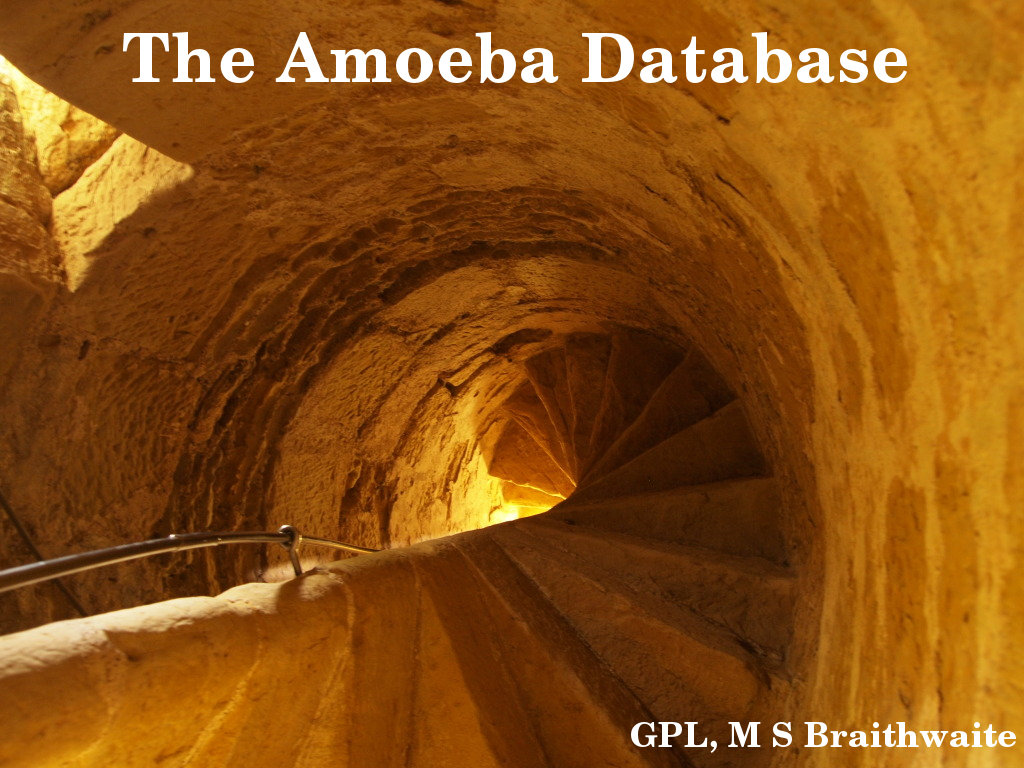
\includegraphics[scale=2]{Amoeba-Cover.jpg}
\end{center}
\noindent
\newline
\newline
\newline
\newline
\newline
\newline
\newline
\newline
\begin{center}
\huge{\color{white} GNU}
\end{center}
\newpage
\pagecolor{white}
\noindent
\newline
\newline
\newline
\newline
\newline
\newline
\newline
\newline
\newline
\newline
\begin{center}
The front cover is a photograph of a spiral staircase, taken inside Bodiam Castle, UK.
\end{center}
\newpage
\thispagestyle{empty}
\setcounter{tocdepth}{2}
\tableofcontents
\newpage
\setcounter{page}{1}
\pagestyle{headings}
\section{About This Document}
\thispagestyle{empty}
\noindent
\newline
\newline
\newline
\newline
\newline
\newline
\newline
\newline
\newline
\newline
\newline
\newline
\newline
\newline
\newline
\newline
\newline
Copyright \textcopyright 2012, Martyn Braithwaite.
\newline
\newline
Permission is granted to copy, distribute and/or modify this document under the terms of the GNU Free Documentation License, Version 1.3 or any later version published by the Free Software Foundation; with no Invariant Sections, no Front-Cover Texts, and no Back-Cover Texts. A copy of the license is included in the section entitled ``GNU Free Documentation License".
\newline
\newline
\newline
\newline
\newline
\newline
\begin{center}
\begin{tabular}{c}
Amoeba documentation version 1.0. \\
This document was typeset in \LaTeX. \\
\end{tabular}
\end{center}
\newpage
\noindent
\section{Abstract}
Existing databases have functional limitations that handicap their application to real world situations. Having to define a schema before provisioning the data introduces unnecessary overhead into deployments, costing time and money. Additionally, databases frequently lack the flexibility during run-time to accept wide ranges of data. 
\newline
\newline
This particular database, was written for ENiX 3, and is an extension to the existing database in ENiX 3 called Working Memory System (WMS). WMS was only intended as a reliable, feature rich data storage mechanism, and had no high performance objectives. The idea to write Amoeba was the product of approximately five years of thought, reflecting on the needs of ENiX 3 and database use in general. I wanted Amoeba to abstract out all the complexity of data storage for operational clarity, and focus on being more flexible in the data that it can store. 
\newline
\newline
It became increasingly apparent that the majority of data stored in ENiX 3, was about graph theory and associative references. Nothing could be a more lucid demonstration of this than the concept of Hidden Markov Models and directed graphs. There was a considerable amount of redundancy of data in WMS which resulted in significant memory wastage in duplication. Furthermore, WMS relied on reading and writing to disk locally at the end of every batch of updates, which is itself inefficient.
\newline
\newline
A major performance flaw of WMS is that it is linked list based, with no indexing, allocation table or no caching mechanism. This becomes computationally expensive when it requires a complete database search to dereference an attribute's equivalence. As the database increases in size the time taken to operate on its contents slows down linearly. 
\newline
\newline
Amoeba addresses all of these issues. Firstly, it is habitually resident in RAM, has threading, networking and locking mechanisms allowing the possibility of utilising local host and network resources more appropriately. Secondly, Amoeba is completely schemaless, it can store any binary data of any length or format and each record stores only one piece of data, its primary key. No attributes are stored in a record, only references to other records. Because the data stored is the primary key, it is not necessary for there to duplication of data within Amoeba. Thirdly, Amoeba is indexed, has an allocation table, aggressive caching behaviour and drastically reduces the need for searching.
\newline
\newline
In summary, Amoeba is a flexible and simple database concept using a novel design, is performant and has some remarkable characteristics. 
\newpage
\noindent
\section{Record Structure}
An amoeba is a unicellular organism. The design principle of an Amoeba record is similar, rather than have the records partitioned into statically sized data areas for attributes to be crammed inside, Amoeba's only data attribute is the name of the record (in binary) which can be any length and is stored as a character array type. The rest of the data in an Amoeba record are references to other records. These references can be dereferenced to attributes. 
\newline
\newline
These references are divided into 4 categories:
\begin{enumerate}
\item \textbf{The reference table:} this is a list of all links everywhere in Amoeba that refers to this record. Each in-bound reference in the reference table also gives the exact location of the out-bound reference that aliases this record as an attribute. This is the only part of a record with in-bound references.
\item \textbf{The header:} taken directly from WMS, the header of a record contains the name of the record, and 7 outbound references to statistics about the history of the record. These statistics are for correctly maintaining the records and determining what the records are used for. 
\item \textbf{Qualifiers:} this section is paired reference by reference to the values section. A qualifier in ENiX defines an aspect of comparison to be qualified by a value (in the values section).
\item \textbf{Values:} this section is paired reference by reference to the qualifiers section. A value in ENiX defines the qualification of a type of comparison, a comparison which is defined in the qualifier section.
\end{enumerate}
\begin{figure}[ht]
\centering
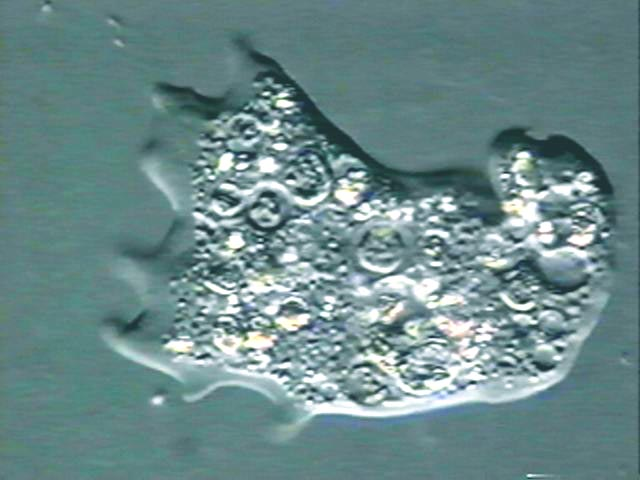
\includegraphics[scale=0.3]{amoeba.jpg}
\caption{A photo of a real life amoeba. Note that it is an irregular shape and the cytoplasm juts out into pseudopods. An amoeba usually has one nucleus, many pseudopods, and many mitochondria per pseudopod with its  cytoskeleton. This anatomy is mirrored in the Amoeba database.}
\end{figure}
\newpage
\noindent
\begin{SCfigure}
\caption{This diagram shows a comparison between an example of a ``typical" database record and an Amoeba record. Note that Amoeba's records have flexibility and are not bounded in size by schema definitions. Note also that there is no data stored in an Amoeba record other than the primary key (grey). The rest of the Amoeba record is populated by inbound and outbound references, both of which have a static size, although the number of them in each section of Amoeba is variable apart from in the header, which has precisely 7. This diagram shows the physical layouts.}
  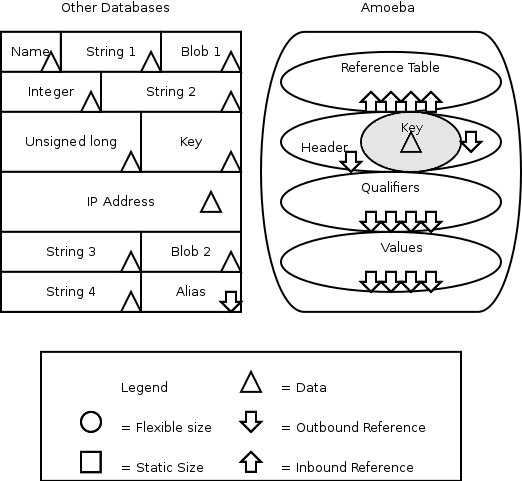
\includegraphics[scale=0.5]{AmoebaRecordStructure.png}
\end{SCfigure}
\begin{figure}[ht]
\centering
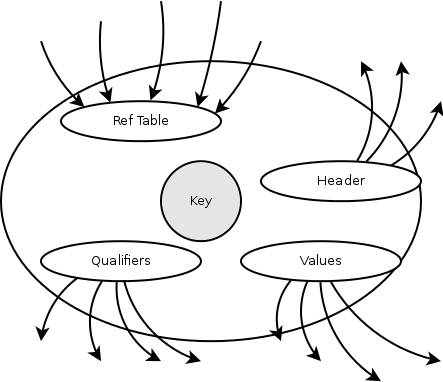
\includegraphics[scale=0.4]{AmoebaRecordStructure2.png}
\caption{A logical diagram of the Amoeba database records. The arrows show inbound and outbound references that connect to the other records. Note that the outbound references only connect to record, whereas the inbound references connect to outbound references within other records. The logical view resembles the anatomy of a neuron.}
\end{figure}
\newpage
\noindent
\section{Memory Structure}
Amoeba uses SHM. To get around the problem of being unable to allocate contiguous memory regions, the SHM is divided up into two sections and allocated separately, this significantly reduces the probability of failure to start up Amoeba. Both halfs are symmetrical in layout. One SHM segment is used for ENiX's data, and the other half for ENiX's methods. It should be reasonably simple to increase or decrease the size and number of SHM segments, if needed, in the future.
\subsection{SHM Segment Header}
This contains basic information about the SHM area, for example:
\begin{itemize}
\item If the segment is locked
\item The number of physical records in the segment
\item The position of end of the record that is closest to the end of the data area in the segment
\item The size of the segment
\item The size of the allocation table
\item The offset relative to the start address of the SHM segment of where to find the allocation table
\end{itemize}
\subsection{Segment Allocation Table}
This section contains information on where to find records in the database quickly. This section is divided into 3 subsections:
\begin{itemize}
\item The start positions of the records, which is an address relative to the offset of the start of the data area of the segment
\item The end positions of the records, again an offset from the start of the data area
\item The cache lookup table, which is a list of records sorted by the most used records first. The dereferenced lookup on a cache entry, returns a position in the allocation table for where to find the record
\end{itemize}
\subsection{Data Area}
Amoeba does not use buckets to contain records. Instead, it tessellates the records adjacently in SHM with no space in between. It never writes before the last written position in the database, unless it is replacing a record which is not bigger than the original it replaces. The database automatically defragments when there is no space left to add more data after the last written position. This eliminates the need to keep a cumulative record of free space within the database and guarantees that the allocation table reflects a total order relation with the positions of data allowing much faster defragmentation.
\newpage
\noindent
A complete diagram of an SHM segment would look something like this:
\begin{figure}[ht]
\centering
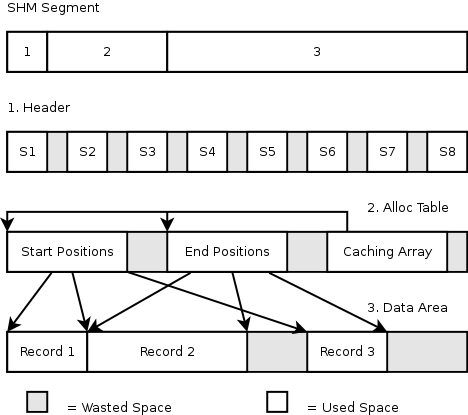
\includegraphics[scale=0.7]{SHMStructure1.png}
\caption{A breakdown of example data allocation with an SHM segment. Data is evenly distributed throughout the header and the allocation table, so there can be a little wasted space here. There can be wasted space in the data area, but only because of fragmentation. The cache maps back to the start and end positions of data in the database, and these point to the start and end positions of records in the data area of the segment.}
\end{figure}
\newpage
\noindent
\section{Amoeba Searches}
\subsection{Amoeba ``Searchless" Data Retrieval}
Searches in databases are computationally expensive, so Amoeba is designed to avoid searches if possible, and to optimise the searches when it isn't. Unfortunately, it is not possible to eliminate searches in a database completely; however, in Amoeba, once a record references another record, it is not necessary to do any further searching.
\newline
\newline
A relative comparison of search characteristics of different database would reveal something a bit like this:
\begin{figure}[ht]
\centering
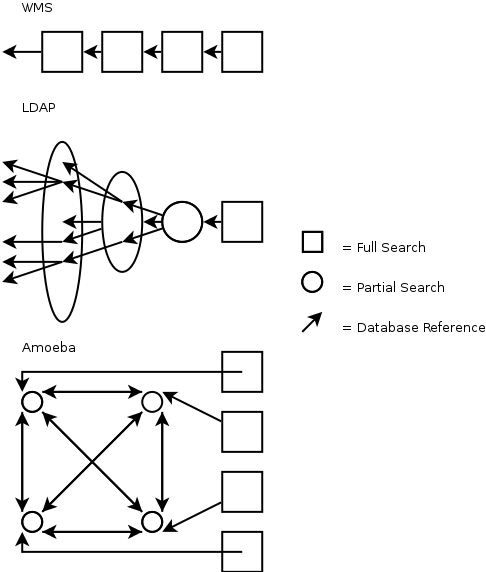
\includegraphics[scale=0.7]{AmoebaSearch1.png}
\caption{A relative view of the searching behaviour of databases. Amoeba shares behaviours in common with LDAP because after the initial full database search, it needs to only search for references locally within a segment of the database. Amoeba however has two major advantages over the directory tree layout. First it is a networked rather than tree layout, allowing better cross record connectivity (eliminating a lot of full database searches in LDAP). Secondly, the number of partial search references can be kept much lower.}
\end{figure}
\newpage
\noindent
\subsection{Geometric Caching}
There may be a number of records that come up frequently, or have been recently used a lot, typically the most used records continue to be most used in the short term. Database searches are extremely computationally expensive. In Amoeba, all record's positions are cached in an array in the allocation table, this is searched from start to finish for records, so to increase the speed of the search on the record, the records cache must be moved closer to the start of the cache. This is done geometrically with ratio, $r={{1}\over{2}}$.
\newline
\newline
If $P_n$ represents the position of the record after n consecutive searches, and $k$ the start position of the record, then: 
$$
P_0=k
$$
After $n$ consecutive searches this becomes:
$$
P_n={{k}\over{2^n}}
$$
Records that take less priority over this record, aren't evicted from cache or swapped with this record, instead they are shifted along away from the start of the cache, so for these records after n consecutive cache misses, their position is:
$$
P_n=k+n
$$
This caching policy gives a fast bias towards caching records that are being used now, yet at the same time, being very reluctant to reduce record's hard earnt cache positions.
\begin{figure}[ht]
\centering
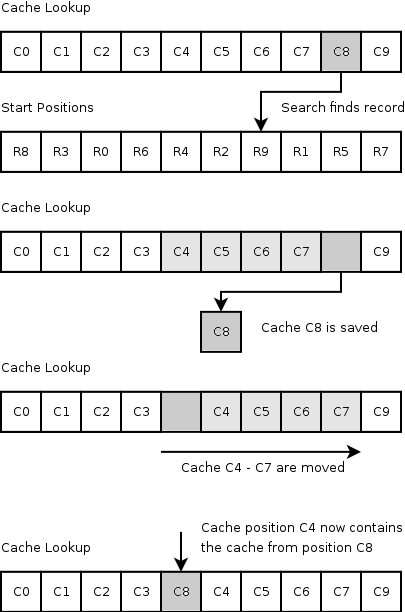
\includegraphics[scale=0.4]{CacheEviction1.png}
\caption{This diagram shows the cache eviction policy for records in cache. The light grey shows the cache being evicted into a low priority, while dark grey shows the found record being promoted so it will be found twice as fast as it was previously in future searches.}
\end{figure}
\newpage
\noindent
\begin{figure}[ht]
\centering
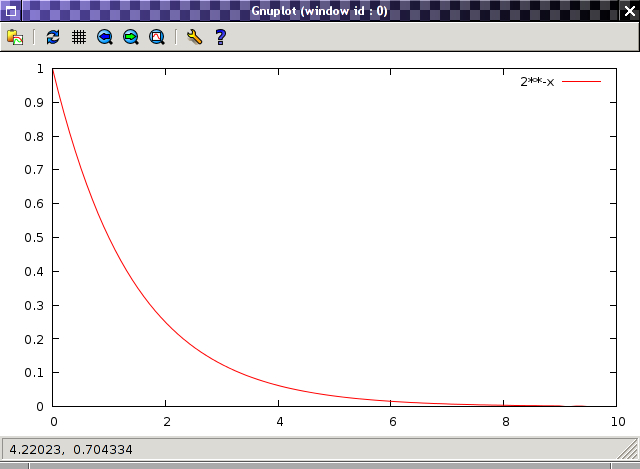
\includegraphics[scale=0.9]{CacheEviction.jpg}
\caption{The graph above shows the time taken to find a record after 10 adjacent recaching attempts. Note the exponential drop in time taken to process the search. In practice the the record is never cached in position 0 of the data area because this is occupied by the BLANK record. }
\end{figure}
\subsection{Process Distribution}
To make better used of localhost CPU resources, Amoeba uses shared memory (SHM), which allows other clients to access to SHM and make modifications to it. Additionally the searches are thread-safe and there is a measurable improvement in the speed of searches when using multiple threads for searching although, although for 2 threads it is only approximately 10-20\% faster than a single thread.
\newline
\newline
If $T_{n}$ is a set of records searched by the nth search thread, the maximum number of threads is $m$ the set $R$ is a list of all records to be searched, then:
$$
T_n= \{\forall r_i \epsilon R: m|(i-n)\}
$$
So approximately ${|m|}\over{n}$ search operations are done by each of the $m$ threads.
\newpage
\noindent
When a record has been found, the search thread uses IPC to signal to the other threads to terminate next time they have CPU time. Visually, if there are 8 records and 3 search threads, then the distribution of record searches would be handled as follows:
\begin{figure}[ht]
\centering
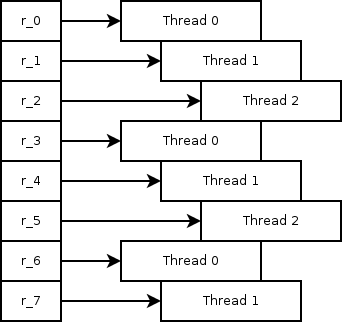
\includegraphics[scale=0.6]{SearchThreads1.png}
\caption{The distribution of records to the search threads follows a round-robin pattern, and the threads search from the start to the end of the cache searching the most used frequently used records first of all.}
\end{figure}
\newpage
\noindent
\section{WMS to Amoeba Translation}
Amoeba records themselves contain no useful information unless the outbound records are dereferenced. This section details how it is possible reassemble and disassemble meaningful data to and from the Amoeba record format. Note that unlike other databases, \emph{Amoeba makes no distinction between attributes and records. They are treated equally and have identical structure and function.}
\subsection{Preparation for Updates}
There are two critical things to do before committing any form of Amoeba modification:
\begin{enumerate}
\item Lock the database from any read or write operations.
\item Re-reading the SHM segment's header (fixed in v1.1).
\end{enumerate}
Most databases implement some kind of locking. Amoeba implements a very simple lock that uses the entire SHM segment as a locking base. This lock prevents any two high level operations that search or modify the database from running concurrently. When two modifications are committed to Amoeba simultaneously, there will be memory corruption due to allocation table changes (from defragmentation), loss of data caused by the allocation table committal race conditions, and search malfunctions caused when searches look for data that has changed or is no longer in the database.
\newline
\newline
Each running Amoeba process that reads the same SHM segments have their own view of the header. The header contains information such as the number of records in the segment and the last position that was written to in the data area. With a multiprocess application, both processes are going to be making individual updates. After any such update, a process will update the header with the new population and the last written position. If a second process fails to re-read this header and it commits an update, it could overwrite some of the changes made by the first process. 
\subsection{Creating Records}
Information is presented to Amoeba in WMS format, so translation is required to convert this format into Amoeba format. This involves:
\begin{enumerate}
\item Creating an Amoeba head record, if it doesn't already exist.
\item Listing all the WMS attributes of the record.
\item Creating a record of each of these attributes, if they don't already exist.
\item Locating the position in the allocation table for each of these records.
\item Creating a outbound reference from the head record to each of the attribute records.
\item Creating inbound references from the attribute references to the reference table of the head record.
\item Committing all modified records to disk.
\end{enumerate} 
\newpage
\noindent
\begin{figure}[ht]
\centering
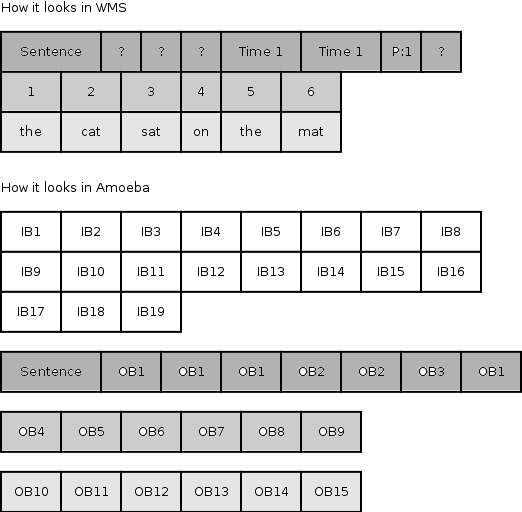
\includegraphics[scale=0.6]{WMS2Amoeba.png}
\caption{This shows how a WMS record looks after it has been translated into Amoeba. IB stands for inbound reference, OB stands for outbound reference. Note that there are only 15 outbound references, but there are 19 inbound references. This is because the outbound references refer to unique records and there are duplicate references, however the inbound references are unique to the positions inside the attribute records. The sections of the record are colour shaded different greys for easy comparison.}
\end{figure}
\newline
The diagram on the next page shows the high level overview of how the this example would look logically.
\newpage
\noindent
\begin{figure}[ht]
\centering
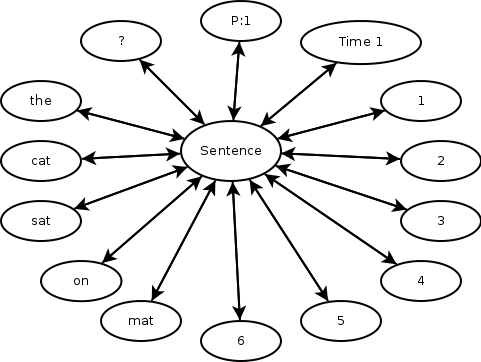
\includegraphics[scale=0.5]{WMS2Amoeba2.png}
\caption{In this figure, the attributes that were in WMS have been removed and translated into separate database records in Amoeba. Instead of storing attributes in the record it stores references to other records which can be dereferenced as attributes. Note again that there is no duplication of data, and that for each outbound reference to the attribute records, there is a inbound reference to the reference table.}
\end{figure}
\subsection{Linking and Delinking}
Correct management of the references between the head record and the attribute records is crucial. Inbound references store information on which records reference this record in their outbound references. Similarly, for outbound references. Associations can be formed and severed. However, if any records are deleted and the outbound references to these records aren't removed, then the references become severed and become hanging references resulting in runtime errors.
\begin{figure}[ht]
\centering
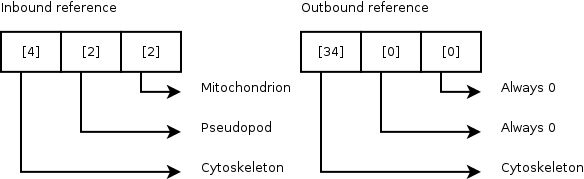
\includegraphics[scale=0.6]{Reference1.png}
\caption{Here are some example references from Amoeba. Outbound references always contain two zeros because they refer to records only. Inbound references come from a outbound reference in another record. It is worth noting that these references are atomic units of data in Amoeba, these triplets are stored in structures called mitochondria. A mitochondrion can be used to search the database and return either another mitochondrion or a record if it is an inbound or outbound reference respectively.}
\end{figure}
\newpage
\noindent
\begin{figure}[ht]
\centering
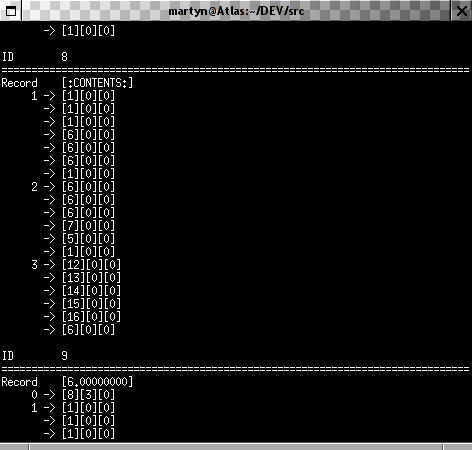
\includegraphics[scale=1]{Reference2.png}
\caption{shows a screenshot of an Amoeba record. On each line is an Amoeba mitochondrion, the ordered triplets we saw earlier. Inbound references are contained in pseudopod 0, pseudopods 1-3 contain outbound references to attribute records in the header, qualifier and values fields respectively.}
\end{figure}
\newline
Inbound and outbound references should only created and destroyed in pairs so that relationships are always bi-directional. When one of two records are deleted, all inbound and outbound mutual relations between objects should be severed first.
\subsection{Deleting}
Once link management in the Amoeba database is understood, removing records is straightforward. A deletion process occurs in the following order:
\begin{enumerate}
\item Collect a list of records that refer to the deleted record.
\item Delete the attribute pairings for those outbound references to the deleted object.
\item The allocation table entry for the deleted object is mapped back to the blank record to indicate it no longer exists.
\end{enumerate}
\newpage
\noindent
\section{Fragmentation}
All data storage mechanisms suffer from the problem of data fragmentation. This occurs when there is unused space between the used data areas. Because the space is not contiguous it can limit the size of data stored in these free space slots. Over time, it becomes inevitable that the fragmentation is so great than even if 50\% of the space is used, there is 0\% unusable space. Amoeba does not defragment as it processes updates, Amoeba defragments when it has run out of space and it does this automatically, often in the middle of an update.
\begin{figure}[ht]
\centering
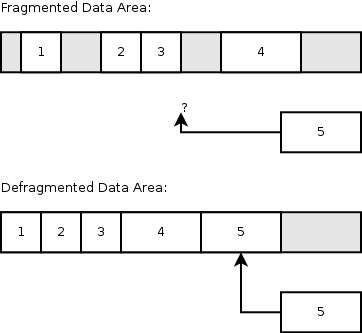
\includegraphics[scale=0.5]{Fragmentation1.png}
\caption{This diagram shows the problem with storage systems when they become fragmented. In the first example there is plenty of free space, but nowhere big enough to store record 5. The second example shows that after the data area is defragmented, not only is there enough space to store record 5, but it has enough free space left over to even store another record of equal size after that. Gray represents free space.}
\end{figure}
\newline
Amoeba suffers from two different types of fragmentation. Allocation table fragmentation and data area fragmentation. 
\subsection{Allocation Table Fragmentation}
Unlike data fragmentation, allocation table fragmentation occurs not when it is unable to write because of space constraints, but when it cannot reuse old allocation table spaces because the algorithm forbids it. Amoeba is an indexed database, where the record's outbound references refer to attribute records. Linking and de-linking these records are computationally expensive, so avoiding this is a priority. Unfortunately, by reusing free allocation table space all records after the newly added record have to be de-linked from the rest of the database and then re-added, because their position changes. So for example, if there are 1000 records after the record being added, placing the new record in the free allocation table space, means that it could take 1000x longer to add than if it just placed it at the end of the allocation table space.
\newline
\newline
The existing approach is to link the allocation table entries for deleted records back to the blank record at the beginning of the data area, then not to reuse this blank space again. When Amoeba has run out of allocation table space, it defragments the allocation table by de-linking the last record in the database, moving it to the first free space and re-linking it in its new position. This continues until there is no fragmentation.
\begin{figure}[ht]
\centering
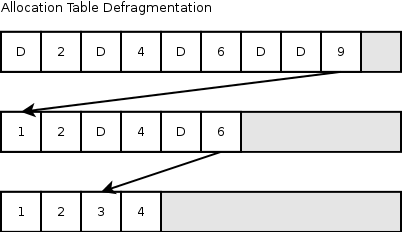
\includegraphics[scale=0.5]{Fragmentation2.png}
\caption{In the allocation table all the entries are the same size, in this example, the grey represents unused space, and D represents deleted records. Records closest to the end of the allocation table are de-linked and moved to overwrite the deleted records. Note that the position of the entries change, justifying the need for re-linking the references. When there are no deleted records left after the last record, all the deleted records are freed leaving free space in the allocation table. Note the numbers indicate the reference position of the record in the allocation table, not the allocation table contents i.e. the position of the record in the data area.}
\end{figure}
\subsection{Data Area Fragmentation}
Before the amount of free space can be calculated, the allocation table has to be defragmented. This is because there may be references to deleted records that link back to the blank record at the start of the segment, and will mean that used space is double counted for blank records. The second thing is to sort out the allocation table contents relative to the start position of records in the data area. Then, in the chronologically sorted records, the fragmentation is given by:
$$
\sum_{i=0}^{n-1}{(S_{i+1}-F_{i})}
$$
Where:
$$
F_{0}=0
$$
And, $F_{i}$ is the finish position of the i-th record, and $S_{i}$ is the start position of the i-th record and $n$ is the number of records in the database.
\newline
\newline
Steps of defragmentation of the data area are:
\begin{enumerate}
\item Defragment the allocation table.
\item Sort allocation table.
\item Where there is a gap, move the next record to the end, repeat until the data area is defragmented.
\item Write all the changed record positions back to the allocation table.
\end{enumerate}
\newpage
\noindent
\begin{figure}[ht]
\centering
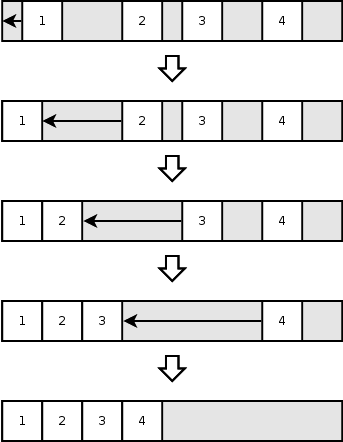
\includegraphics[scale=0.5]{Fragmentation3.png}
\caption{A diagram showing how a simple data area is defragmented. The grey areas are free space, and the numbered boxes are the Amoeba records. This process is O(n).}
\end{figure}
\section{Properties}
Amoeba database features the following properties:
\begin{itemize}
\item Records and attributes are the same
\item Renaming an attribute record renames all the attributes in the database in one operation
\item Only the primary key is stored in a record
\item The primary key and the name of the record is the same
\item No duplication of data occurs
\item Amoeba can be easily made to appear as another other database
\end{itemize}
\newpage
\noindent
\section{Performance}
Testing and development was conducted on a HP 6930p Elitebook with a 2.53 GHz Core2Duo and 8GB of RAM, and a HP zx6000 2x 1.4Ghz IA64 with 4GB of RAM.
\newline
\newline
At the time of writing this document, on 2x 10,485,760 byte SHM segments Amoeba database with 2 threads enabled and a 3,000,000 byte allocation table in each segment:
\newline
\begin{center}
\begin{tabular}{r || r | r || c}
%%\hline
\rowcolor[gray]{0.8}
Test & 6930p & zx6000 & Test Code\\
%%\hline
Read from disk &417 ms&&-\\
Write to disk &401 ms& &-\\
Create blank database &22 ms& &-\\
Search 100k Amoeba records &2974 ms&&s \\
Delete and add 100k Amoeba records &880 ms&&d \\
Modify 100k Amoeba records &837 ms&&m \\
Write 999 WMS records &950 ms&&W \\
Read 999 WMS records &9 ms&&Ww*\\
Defrag alloc table of 999 records&3 ms&&WWD\\
Full defrag of 999 records&9 ms&&WWF\\
%%\hline
\end{tabular}
\newline
\newline
*\emph{Modified so that the records were not displayed only translated into WMS.}
\end{center}
\noindent
\newline
These performance tests were carried out with the assistance of Amoeba-DEBUG which is an Amoeba unit testing framework.
\newpage
\noindent
\section{Logging}
The Amoeba daemon process logs the most important timestamped events to the console like this:
\begin{center}
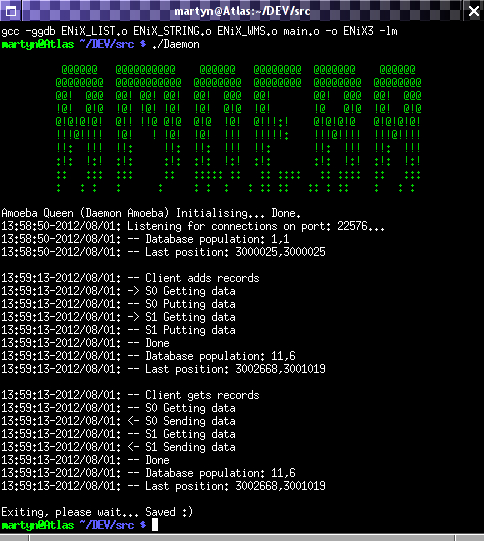
\includegraphics[scale=1]{Amoeba-Logging1.jpg}
\end{center}
\noindent
In the event of malfunction or questionable behaviour, it is possible to attach the Amoeba-DEBUG binary to the running Daemon process, and this shell can be used to debug the database contents and issue test cases for fault reproduction. Note that suspicious behaviour will be logged to the console as flashing text.
\section{Usage}
Running the Amoeba Daemon process is as simple as executing ./Daemon, this will setup SHM and listen to incoming connections on port 22576. The Amoeba-API.c contains a framework of functions that can be used to meaningfully communicate to and from the daemon process. When the daemon is no longer needed, it can be Ctl-C'd or sent a kill signal, the Daemon will trap the signal and exit, saving the database to disk.
\newpage
\noindent
\begin{center}
\begin{tabular}{l  r }
\rowcolor[gray]{0.8}
Component & function\\
\rowcolor[gray]{0.9}
ENiX\_STRING & ENiX's string processing library\\
\rowcolor[gray]{0.9}
ENiX\_LIST & ENiX's list processing library \\
\rowcolor[gray]{0.9}
ENiX\_WMS & ENiX's Working Memory System model \\
\rowcolor[gray]{0.9}
WitchCraft-Colours & WitchCraft's ASCII colour library\\
\rowcolor[gray]{0.9}
WitchCraft-Net & The WitchCraft networking library\\
Amoeba-API & The API that controls Amoeba\\
Amoeba-Colony& Amoeba components that communicate with SHM \\
Amoeba-Cytoskelenton& Amoeba record construction functions \\
Amoeba-Daemon&Amoeba Daemon specific functions \\
Amoeba-Microtubules&Functions to translate between WMS and Amoeba \\
Amoeba-Nucleus&Amoeba handler library \\
Amoeba-Test&The Amoeba-DEBUG shell \\
Amoeba-Unit-Tests& Functions called by Amoeba-DEBUG shell \\
%%\hline
\end{tabular}
\end{center}
\noindent
\newline
New functions should be added to Amoeba-API if required. It should not be necessary to modify the other libraries unless there is a fault. Light grey indicates libraries that are imported from ENiX for compatibility and are not really part of Amoeba.
\section{Improvements}
Some improvements that could be added to the Amoeba database without too much difficulty.
\begin{itemize}
\item Link the header data directly with the SHM to reduce overhead and the requirement to constantly reread the header. 
\item Check if there is a workaround for allocation table fragmentation. 
\item Optimise the WMS - translation process.
\item Permissions could be added through an additional API.
\item System redundancy and distribution of Amoeba records via multiple databases could be possible using an Amoeba proxy with hash table record distribution, increasing speeds by orders of magnitude.
\item Extend Amoeba into a networked filesystem.
\item Plugins to allow Amoeba to emulate other database appearances. 
\end{itemize}
\newpage
\noindent
\thispagestyle{empty}
\pagestyle{empty}
\pagecolor{black}
.
\end{document}
